\chapter{the theory of simple gases}
\section{an ideal gas in various quantum-mechanical ensembles}
\subsection{in a microcanonical ensemble}
\begin{itemize}
	\item 用能级 $\epsilon_i$ (不是能量本征态) 上的粒子数 $n_i$ 表示系统的状态 $\{n_i\}$, 有
	\begin{equation}
		\begin{dcases}
			\sum_i n_i = N \\
			\sum_i n_i \epsilon_i = E
		\end{dcases},
	\end{equation}
	系统的微观状态数为
	\begin{equation}
		\begin{dcases}
			W_\text{B}\{n_i\} = \prod_i \frac{(n_i + g_i - 1)!}{n_i! (g_i - 1)!} \\
			W_\text{F}\{n_i\} = \prod_i \frac{g_i!}{n_i! (g_i - n_i)!} & n_i \leq g_i
		\end{dcases},
	\end{equation}
	其中 $g_i$ 表示粒子的 $\epsilon_i$ 能级的 degeneracy.
	\begin{itemize}
		\item 用 Stirling 公式作近似,
		\begin{equation}
			\begin{dcases}
				\ln W_\text{B}\{n_i\} \approx \sum_i \Big( (n_i + g_i) \ln(n_i + g_i) - n_i \ln n_i - g_i \ln g_i \Big) \\
				\ln W_\text{F}\{n_i\} \approx \sum_i \Big( g_i \ln g_i - n_i \ln n_i - (g_i - n_i) \ln(g_i - n_i) \Big)
			\end{dcases}.
		\end{equation}
	\end{itemize}
	
	\begin{tcolorbox}[title=calculation:]
		对于 Bose-Einstein statistics, 往 $g_i$ 个格子中放 $n_i$ 个 indistinguishable 小球, 有
		\begin{equation}
			\begin{dcases}
				\frac{g_i^{n_i}}{n_i!} & \text{一个格子放多个球的情况可忽略时, 即} \ g_i \gg n_i \\
				\frac{(n_i + g_i - 1)!}{n_i! (g_i - 1)!} & \text{插板法}
			\end{dcases}
		\end{equation}
		种放法. 插板法: 球 ($n_i$ 个) 和板 ($g_i - 1$ 个) 都是 indistinguishable, 它们各自可以放在 $(n_i + g_i - 1)!$ 个位置...
		
		\noindent\rule[0.5ex]{\linewidth}{0.5pt} % horizontal line
		
		对于 Fermi-Dirac statistics, 每个格子最多一个小球, 有
		\begin{equation}
			\frac{g_i!}{n_i! (g_i - n_i)!}
		\end{equation}
		种放法.
	\end{tcolorbox}
	
	\item 最概然分布为
	\begin{equation}
		\begin{dcases}
			n_i^* = \frac{g_i}{e^{\alpha + \beta \epsilon_i} - 1} & \text{Bose-Einstein} \\
			n_i^* = \frac{g_i}{e^{\alpha + \beta \epsilon_i} + 1} & \text{Fermi-Dirac}
		\end{dcases},
	\end{equation}
	此时
	\begin{equation}
		\ln W\{n_i^*\} = \alpha N + \beta E - \frac{1}{\eta} \sum_i g_i \ln \Big( 1 - \eta e^{- \alpha - \beta \epsilon_i} \Big), \quad \text{with} \quad \eta = \begin{dcases}
			+ 1 & \text{Bose-Einstein} \\
			- 1 & \text{Fermi-Dirac} \\
			\rightarrow 0 & \text{Boltzmann}
		\end{dcases},
	\end{equation}
	其中 $\alpha = - \beta \mu$.
	
	\item 注意 $P V = T S - U + \mu N$, 得到
	\begin{equation}
		P V = - \frac{1}{\eta} k_B T \sum_i g_i \ln \Big( 1 - \eta e^{- \alpha - \beta \epsilon_i} \Big) \overset{\eta \rightarrow 0}{=} N k_B T.
	\end{equation}
\end{itemize}

\subsection{in a canonical ensemble}
\begin{itemize}
	\item 系统的 partition function 为
	\begin{equation}
		Z_\text{C} = \sum_{\{n_i\}} W\{n_i\} e^{- \beta E\{n_i\}},
	\end{equation}
	求和需要满足 $\sum_i n_i = N$ 的约束条件, 不方便处理, 这个约束在 grand canonical ensemble 中不存在.
\end{itemize}

\subsection{in a grand canonical ensemble}
\begin{itemize}
	\item 系统的 grand partition function 为
	\begin{equation}
		Z_\text{GC} = \sum_{\{n_i = 0\}}^{\{n_i = \text{max}\}} W\{n_i\} e^{- \beta E\{n_i\} - \alpha N\{n_i\}} = \begin{dcases}
			\prod_i (1 - e^{- \alpha - \beta \epsilon_i})^{- g_i} & \text{Bose-Einstein} \\
			\prod_i (1 + e^{- \alpha - \beta \epsilon_i})^{g_i} & \text{Fermi-Dirac} \\
			\prod_i \exp \Big( g_i e^{- \alpha - \beta \epsilon_i} \Big) & \text{Boltzmann}
		\end{dcases},
	\end{equation}
	它们的函数图像分别为如下图 (观察到 $\epsilon$ 越大 (等价于 $\beta$ 越大), 三种统计的差别越小; $g$ 显然没有影响):
	
	\begin{figure}[H]
		\centering
		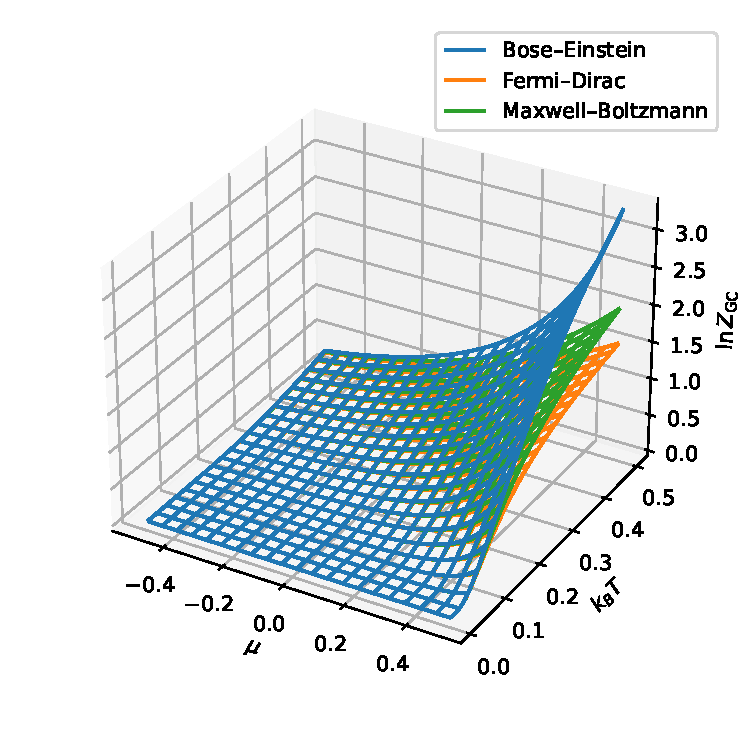
\includegraphics[scale=0.75]{figures/grand partition functions with g = 3, epsilon = 0.7.pdf}
		\caption{grand partition functions with $g = 3, \epsilon = 0.7$.}
	\end{figure}
	
	\begin{tcolorbox}[title=calculation:]
		对 Bose-Einstein statistics,
		\begin{equation}
			Z_\text{GC} = \prod_i \sum_{n_i = 0}^\infty \frac{(n_i + g_i - 1)!}{n_i! (g_i - 1)!} (e^{- \alpha - \beta \epsilon_i})^{n_i},
		\end{equation}
		注意到 Taylor expansion
		\begin{equation}
			\frac{1}{(1 - x)^n} = \sum_{m = 0}^\infty \frac{1}{m!} \frac{(n + m - 1)!}{(n - 1)!} x^m,
		\end{equation}
		所以
		\begin{equation}
			Z_\text{GC} = \prod_i (1 - e^{- \alpha - \beta \epsilon_i})^{- g_i}.
		\end{equation}
		
		\noindent\rule[0.5ex]{\linewidth}{0.5pt} % horizontal line
		
		对于 Fermi-Dirac statistics,
		\begin{equation}
			Z_\text{GC} = \prod_i \sum_{n_i = 0}^{g_i} \frac{g_i!}{n_i! (g_i - n_i)!} (e^{- \alpha - \beta \epsilon_i})^{n_i},
		\end{equation}
		注意到
		\begin{equation}
			(1 + x)^n = \sum_{m = 1}^n \frac{1}{m!} \frac{n!}{(n - m)!} x^m,
		\end{equation}
		所以
		\begin{equation}
			Z_\text{GC} = \prod_i (1 + e^{- \alpha - \beta \epsilon_i})^{g_i}.
		\end{equation}
		
		\noindent\rule[0.5ex]{\linewidth}{0.5pt} % horizontal line
		
		对于 Maxwell-Boltzmann statistics,
		\begin{align}
			Z_\text{GC} &= \prod_i \sum_{n_i = 0}^\infty \frac{g_i^{n_i}}{n_i!} (e^{- \alpha - \beta \epsilon_i})^{n_i} \notag \\
			&= \prod_i \exp \Big( g_i e^{- \alpha - \beta \epsilon_i} \Big).
		\end{align}
	\end{tcolorbox}
	
	\item 得到
	\begin{equation}
		\begin{dcases}
			\Phi_\text{G} = - k_B T \ln Z_\text{GC} \\
			U = \sum_i \frac{g_i \epsilon_i}{e^{\alpha + \beta \epsilon_i} - \eta} \\
			N = \sum_i \frac{g_i}{e^{\alpha + \beta \epsilon_i} - \eta} \\
			S = k_B \Big( \beta U + \alpha N + \ln Z_\text{GC} \Big)
		\end{dcases}.
	\end{equation}
\end{itemize}
